%% !TEX TS-program = pdflatexmk
%% !BIB TS-program = bibtex

\documentclass[12pt, a4paper, oneside]{book}
\usepackage{import}
\subimport{../}{preamble}
\ExecuteBibliographyOptions{articletitle=false}
\standalonetrue
\onehalfspacing
\begin{document}

\begin{singlespace}
\color{white}
\chapter{Conclusions and Outlook}
\end{singlespace}

\AddToShipoutPictureBG*{ \AtPageUpperLeft{ \put(0,-225)
{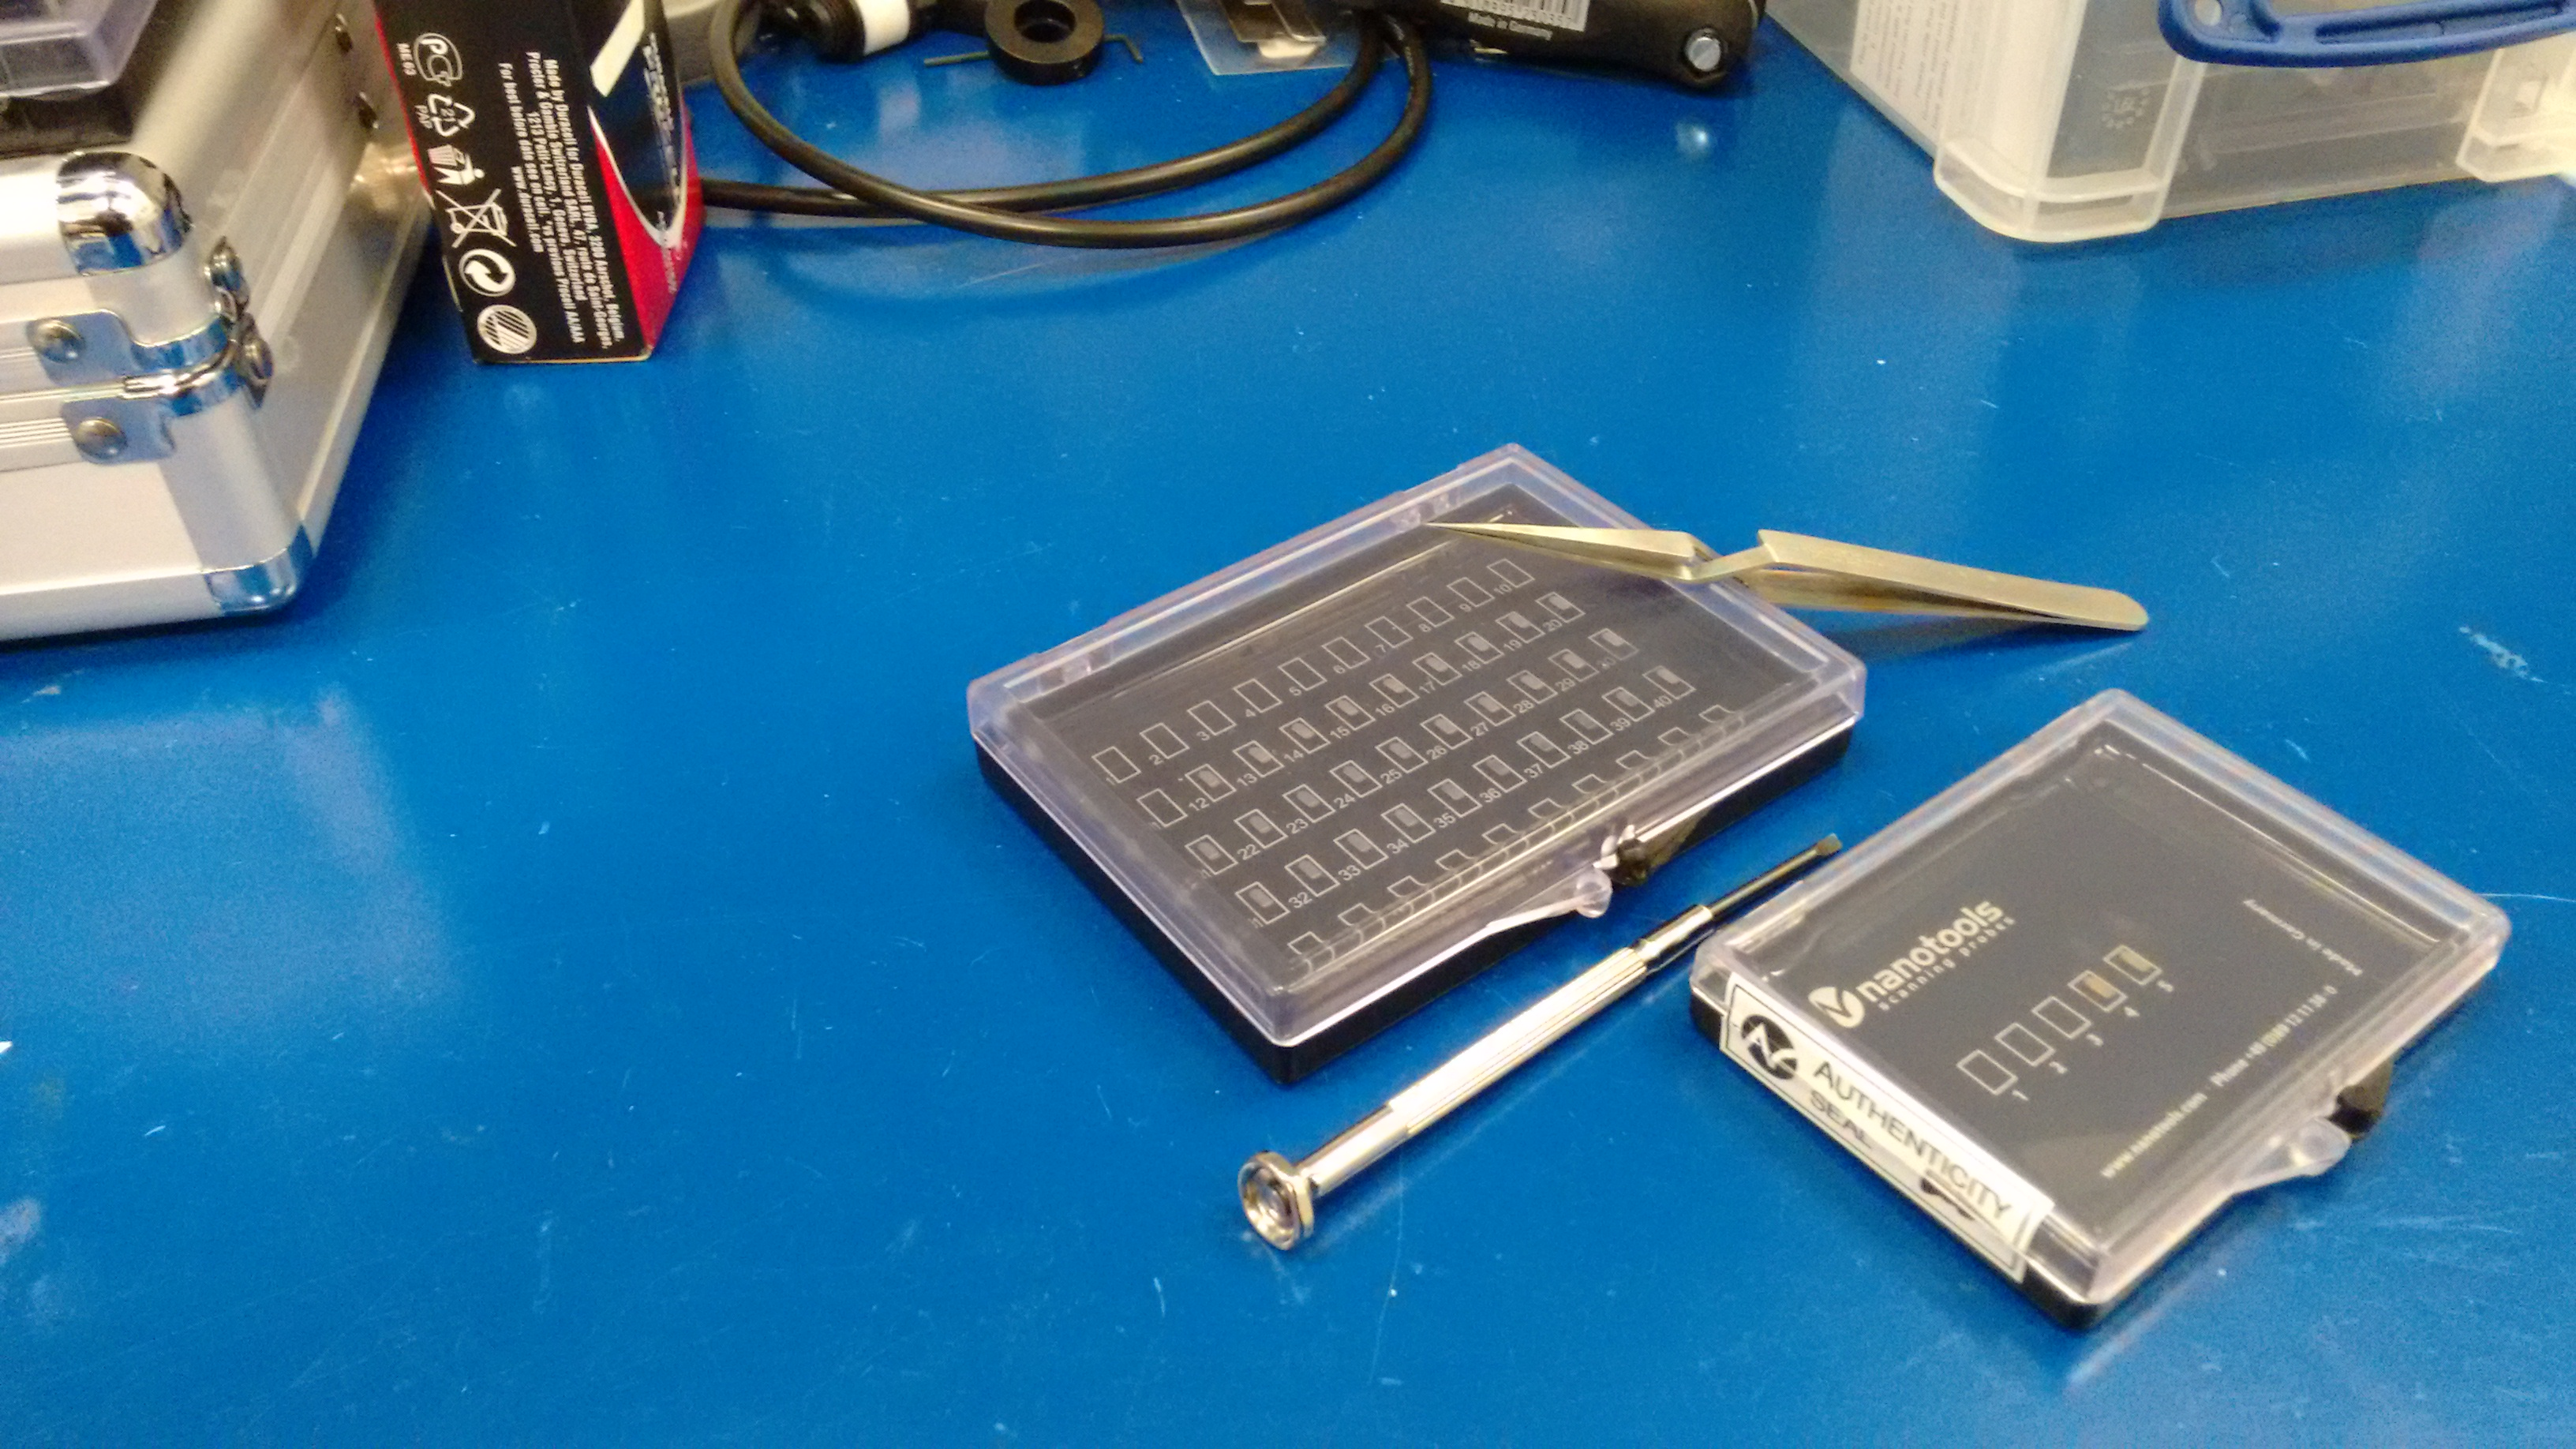
\includegraphics[width=\paperwidth, clip=true, trim=0 80 0 0]{figures/chapter_cover.jpg}}
}}

% Project overview
This thesis has focussed on the understanding and application of tips for plasmonics, with the aim to use tips to further understand the recently revealed sub-nm regime of plasmonic coupling. Though the initial motivation was to investigate quantum regime plasmonics, the project diversified into studying the optical differences between sharp and spherical tips using techniques such as hyperspectral imaging and plasmon coupling, the development of an electrochemical method as an alternative approach to producing spherical tips and the application of plasmonic tips for \gls{ters}. Finally, spherical tips were applied to investigating quantum effects in the sub-nm plasmonic coupling regime. Work was therefore split between three core areas: development of plasmonic tips, design and construction of a custom microscope for tip experiments, and ultimately performing experiments on the combined tip systems.

% Review of spherical tip fabrication
Failure to observe any plasmonic behaviour in the optical far-field spectra of sharp Au \gls{afm} tips, despite their prominence in many near-field enhancing techniques, led to the investigation into nanostructured tip geometries. By nanostructuring an \gls{afm} tip some of the well-known antenna-like properties of isolated plasmonic nanoparticles are transferred into the \gls{afm} probe form factor. Knowing that the particular tip nanostructure and optical geometry set which plasmons exist, and can be experimentally observed, the spherical geometry was chosen for its simplicity. Both commercial spherical Au tips, used in previous tip plasmonics experiments, and AuNP-on-Pt tips, fabricated in-house using a newly developed pulsed electrodeposition procedure, were studied. Pulsed electrodeposition was chosen for its ability to exploit the sharp apex of AFM tips and quickly produce nanostructured tips. The technique was developed from the conception of the idea through to the optimisation of each of the parameters in order to improve reliability with the aim to controllably produce spherical metallic tips. Due to time constraints and the significant effort required to complete other aspects of this project, the controllable growth of spherically-tipped AFM probes through pulsed electrodeposition was only partially achieved. Though certainly not perfected, the technique produced enough samples to {\color{red}accommodate/facilitate} experimentals.
% Work still needed on spherical tip fabrication
Further work is still needed to understand the exact mechanism by which nanoparticles nucleate and grow at and around the apex and complete the optimisation of each growth parameter. Achieving this would enable a large number of varied studies into the application of plasmonic tips for \gls{tenom} - a direction of research only touched upon during this project.

% Review of test rig design chapter
To study the properties of tips and achieve dynamic probing of plasmonic coupling through each interaction regime necessitated the design of a custom microscope capable of combining the function and stability of two opposing AFM devices with a platform for broadband dark-field spectroscopy. The novel design and robust performance of the microscope has been discussed at length and quantified where appropriate. The comprehensive design of the dual-tip platform meant experiments could implement optical, electronic and force measurements for a more complete characterisation of a plasmonic system than is capable in many other experimental setups. Specifically, the combination of hyperspectral imaging and scanning capacitance microscopy enabled the alignment of AFM tips to the focus of the incident beam and to each other, resulting in a highly reproducible dimer plasmonic arrangement. Additionally, the modular design of the microscope and its array of possible measurements make it adaptable and extensible for many other (future) experiments. Within the scope of this project its main use has been to perform experiments on spherical metallic tips.

% Review of tip plasmonics chapter
Observations of strong resonances in spherical metallic tips suggested plasmonic behaviour - an expected feature not found in sharp metallic tips. The agreement between apex spectra extracted from hyperspectral imaging, tuneable \gls{sers} and dynamic plasmon coupling experiments confirm that spherical metallic tips support antenna-like \gls{lsp} modes similar to those in an individual \gls{mnp}, while sharp metallic tips remain unresponsive to light. The spherical Au tip \gls{spr} conveniently exists at the commonly used HeNe wavelength leading to a strongly enhanced Raman response. The measured 30$\times$ improvement in Raman enhancement when using spherical Au tips over sharp Au tips is an advance for \gls{tenom} in the instance of using far-field excitation and detection and a step towards promoting controllable as opposed to randomised nanostructuring. It also suggests that controllable nanostructuring may be the future of \gls{tenom} and bringing about reliable, reproducible single molecular sensitivity. However, without higher quality measurements for direct comparison with evanescent excitation methods, this is only speculation.

% Work still needed on tip plasmonics
Though the results presented within this project only focus on large, spherical Au tips, the developed fabrication and characterisation techniques are not limited to a specific metal or geometry. It would be interesting to measure and quantitatively compare the scattering response of spherical tips with carefully controlled sphere and neck sizes to validate theoretical predictions, and other sphere materials such as Ag, Cu or Al, if such material tips electrochemically deposit in a similar manner to Au. \Gls{ters} could then be carried out on resonance with each type of tip to confirm plasmonic enhancement. A small amount of work was started, with some success, applying pulsed electrodeposition to deposit metal nanostructures other than Au on other conductive \gls{afm} tips, such as highly-doped Si. If successful this would facilitate the production of plasmonic probes resonant across a wide range of visible-NIR frequencies.

% Review of quantum tunnelling chapter
The final sets of measurements used pairs of spherical tips to target the sub-nm coupling regime. The onset of quantum tunnelling and its effects on plasmonic coupling were investigated in ambient conditions, following on from the experiment performed by Savage \emph{et al.} \cite{savage2012} prior to this project. Though the experiment conceptually appears similar, the addition of tunnelling conduction and gap force measurements greatly increased the amount of information that could be extracted to understand the physics of sub-nm gaps. The robust design of the microscope platform enabled many successful scans through the quantum tunnelling regime, observing a slightly different coupling behaviour in each case. Measurements showed both bonding mode screening and \gls{ctp} formation correlated with the onset of quantum tunnelling, though correlation between the two effects differed significantly between different pairs of tips. This is attributed to differences in the gap morphology with the hypothesis that overlap between the plasmonic field and the tunnelling current sets the observed phenomenon. Though still requiring theoretical {\color{red}reassurance/evidence}, this statement implies that atomic scale defects, and the thermal motion of atoms in intense fields have to be considered when designing a plasmonic system.

\subsection{Outlook and Future Directions}

The experiments carried out have both demonstrated the appeal of nanostructured tips and expanded upon the rich regime of tunnelling plasmonics for further exploration. The project leaves at a pivotal point at which atomic-scale morphology and quantum effects have been shown to strongly influence the plasmons confined to a sub-nm gap between metallic surfaces. Within the current system there is still a large amount of scope for further projects. Many questions still remain unanswered for both classical and quantum coupling regimes.

% Parameters not checked in current experiments
Though the mechanisms for varying the humidity are in place, its effects on the tunnelling current and plasmons have yet to be systematically studied. Experiments were typically ran in low humidity environments to reduce adhesion forces caused by the water meniscus, however increased water in the gap is thought to extend the tunnelling regime to larger separations. Conversely, since water always exists in ambient gaps and plasmons can be considered to be tightly confined in sub-nm cavities, it may be the case that the ambient tunnelling regime is completely submerged regardless of non-zero humidity levels. It would therefore be a relatively simple extension to current procedures to attempt multiple repeated scans at different humidity levels under the assumption that the gap morphology is unchanged between scans. Modification of the experiment top chamber could also potentially allow for experiments under vacuum conditions.

The influence of the applied d.c.\ bias on the coupled plasmons has been so far ignored due to the assumption that only optical frequency effects matter. However, it has been suggested that the non-linear nature of electron tunnelling means a strong d.c. bias can be used to tune plasmon coupling \cite{}. Strong biases could also be used to electrically excite coupled plasmons, which could be monitored dynamically to probe the tunnelling regime with a background-free signal.

% Conduction mechanism
Beyond electron tunnelling is the dependence of plasmon coupling on other conduction mechanisms that result from the placement of material in the gap. The effects of conduction on plasmonic hot spots is particularly important to understand since this is the plasmonic geometry recently opted for in techniques like \gls{sers}. The introduction of a gap layer could be used to controllably modify the charge transfer mechanism, as has been successful in nanoparticle systems \cite{benz2014}. Using the current setup it would be possible to measure the influence of different conduction mechanisms on plasmon coupling across a range of spatial regimes. By coating the tips of a dual-tip plasmonic dimer with dielectric, semiconducting, low-dimensionality or quantum materials, their coupling with plasmons can be directly observed, along with their response to both applied biases and strain. The backside of a cantilever or a flat cantilever could even be exploited for high-quality monolayer deposition with plasmons coupling to an image charge \cite{mertens2013, benz2014}. In the event that a spacer material could be externally controlled, e.g.\ through the application of a voltage, the basis for a plasmonic switch could be conceived.

% Why should people be interested
To conclude, the boundary between the capacitive coupling and charge transfer regimes of plasmonics has only recently become accessible, displaying a wealth of interesting physics in only a short period of time. Dynamically controlling the particle positions of an \gls{afm} tip dimer has become a powerful technique for the study of such physics and the results provided by it are expected to be of great interest to the general plasmonic community. From the point of view of fundamental plasmonics, they provide an insight into a largely unknown regime of plasmonics whilst from an applied aspect they indicate the limitations of plasmonics.

\ifstandalone
\begin{singlespace}
\fontsize{8pt}{1em}\selectfont
\printbibliography[notcategory=fullcited]
\end{singlespace}
\fi

\end{document}